% 7. Zusammenfassung
\chapter{Summary}
\label{chap:summary}
This chapter provides a summary of the concept shown in chapter \ref{chap:conceptual-design} and the implementation thereof in chapter \ref{chap:implementation}.

\section{Requirements Engineering}
\label{sec:summary-requirements-engineering}

\section{Concept}
\label{sec:summary-concept}
\emph{TBD:}
\begin{itemize}
    \item \emph{Pipelines + \acp{FSM} lead to tricky debugging. Decouple them and introduce a queue (+metadata) per connection.}
\end{itemize}

\section{Implementation}
\label{sec:summary-implementation}

\begin{figure}[h]
    \centering
    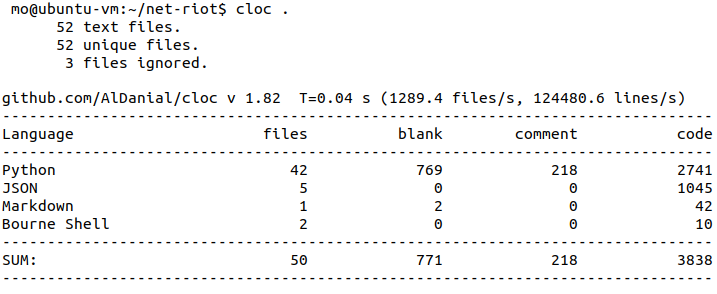
\includegraphics[width=12cm]{img/ch06/cloc.png}
    \captionof{figure}{?} %TODO: Describe
    \label{fig:cloc}
\end{figure}
\emph{TBD:}
\begin{itemize}
    \item \emph{Discuss technical debt!}
    \item \emph{Large config files: bad usability, also confusing}
\end{itemize}